\documentclass{article}

\usepackage{polski}
\usepackage[utf8]{inputenc}
\usepackage{indentfirst}
\usepackage{color}
\usepackage{graphicx}

\newcommand{\TODO}[1]{\textcolor{blue}{TODO: #1}}
\newcommand{\ang}[1]{ang.~{\itshape #1}}

\begin{document}

\title{Metody odkrywania wiedzy \\%
{\large Klasyfikacja -- dokumentacja końcowa} }

\author{Jakub Cichanowicz \and Artur Sawicki}

\maketitle

\section{Analiza i przygotowanie danych}
Zbiór danych składa się z 12 atrybutów. Część z nich ma braki, które należy uzupełnić, gdyż nie wszystkie algorytmy radzą sobie z brakami danych.

\subsection{Klasa pasażerska}

Atrybut ten nie ma braków danych. Rozkład przedstawia się następująco:
\begin{center}
    \begin{tabular}{| l | l | l |}
    \hline
	1   & 2  & 3 \\ \hline
    216 & 184 & 491 \\
    \hline
    \end{tabular}
\end{center}

Z poniższego wykresu można wywnioskować, że atrybut ten miał wpływ na przeżycie.\\
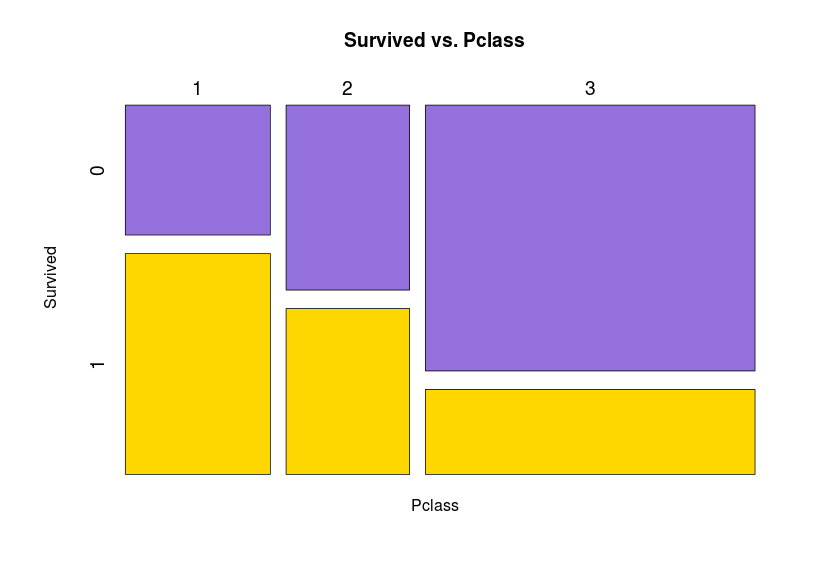
\includegraphics[scale=0.4]{images/survived-vs-pclass.png}

\subsection{Płeć}

Atrybut ten również nie ma braków, a rozkład przedstawia się następująco.
\begin{center}
    \begin{tabular}{| l | l |}
    \hline
	female &  male \\ \hline
	314  &  577 \\
    \hline
    \end{tabular}
\end{center}

Poniższy wykres pokazuje, że płeć ma wpływ na przeżycie.
\begin{center}
	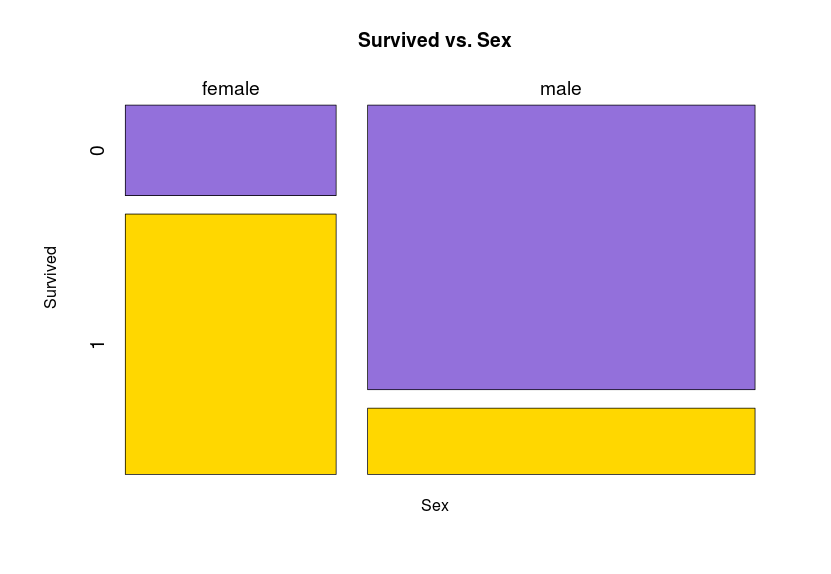
\includegraphics[scale=0.40]{images/survived-vs-sex.png}
\end{center}

\subsection{Wiek}

Wiek jest atrybutem numerycznym o rozkładzie:
\begin{center}
    \begin{tabular}{| l | l | l | l | l | l | l |}
    \hline
Min. & 1st Qu. & Median   & Mean & 3rd Qu.  &  Max.  &  NA's  \\ \hline
0.42  & 20.12  & 28.00  & 29.70 &  38.00  & 80.00   &  177 \\
    \hline
    \end{tabular}
\end{center}

Wykres przedstawiony poniżej pokazuje, że wiek nie wpływa w oczywisty sposób na przeżywalność.

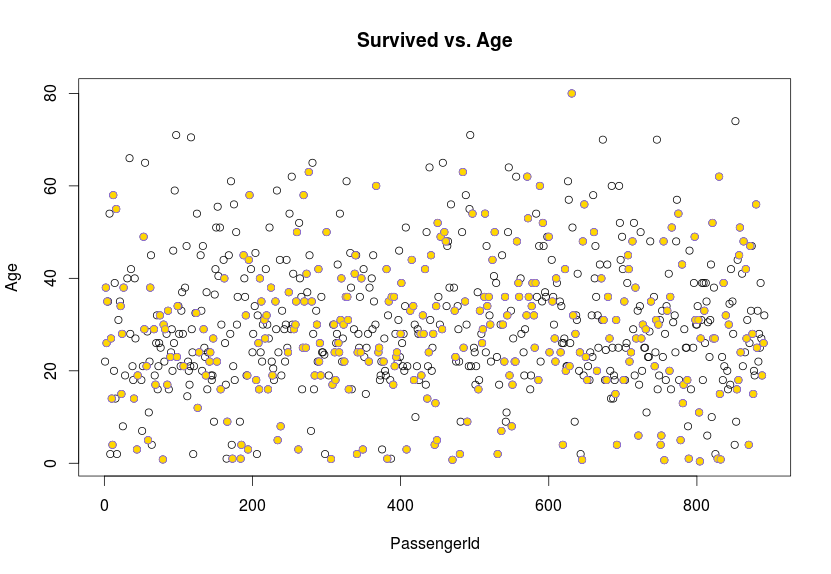
\includegraphics[scale=0.40]{images/survived-vs-age.png}

Braki danych zastąpione zostały w eksperymentach medianą dla płci.

\subsection{Liczba rodzeństwa/małżonków na pokładzie}

Nie ma braków danych. Rozkład przedstawia się następująco:
\begin{center}
    \begin{tabular}{| l | l | l | l | l | l | l |}
    \hline
0 &  1  & 2  & 3  & 4 &  5 &  8  \\ \hline
608 & 209 & 28 & 16 & 18 &  5 &  7 \\
    \hline
    \end{tabular}
\end{center}

Wykres pokazuje, że wpływ atrybutu nie jest jednoznaczny.

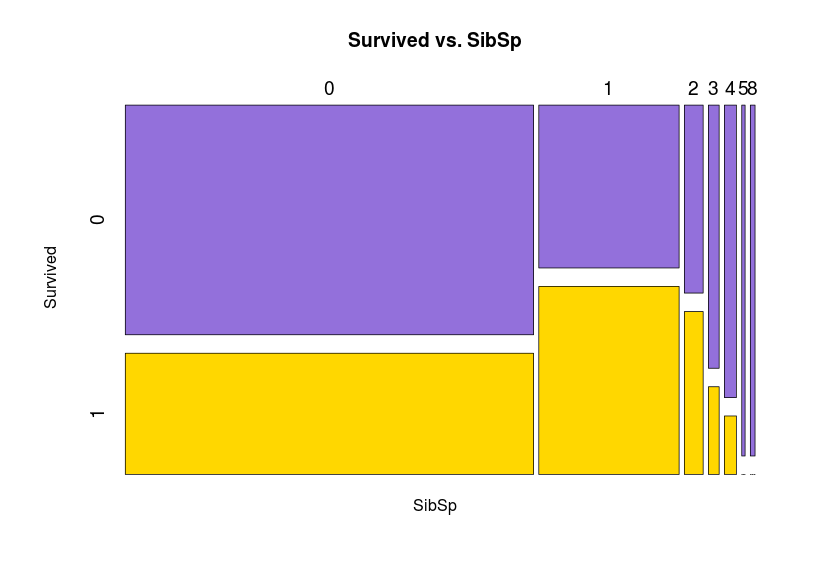
\includegraphics[scale=0.40]{images/survived-vs-sibsp.png}

\subsection{Liczba dzieci/rodziców na pokładzie}

Nie ma braków danych. Rozkład przedstawia się następująco:
\begin{center}
    \begin{tabular}{| l | l | l | l | l | l | l |}
    \hline
 0  & 1  & 2 &  3  & 4 &  5  & 6 \\ \hline
 678 & 118 & 80 &  5  & 4  & 5 &  1 \\
    \hline
    \end{tabular}
\end{center}

Wykres pokazuje, że wpływ atrybutu nie jest jednoznaczny.
\begin{center}
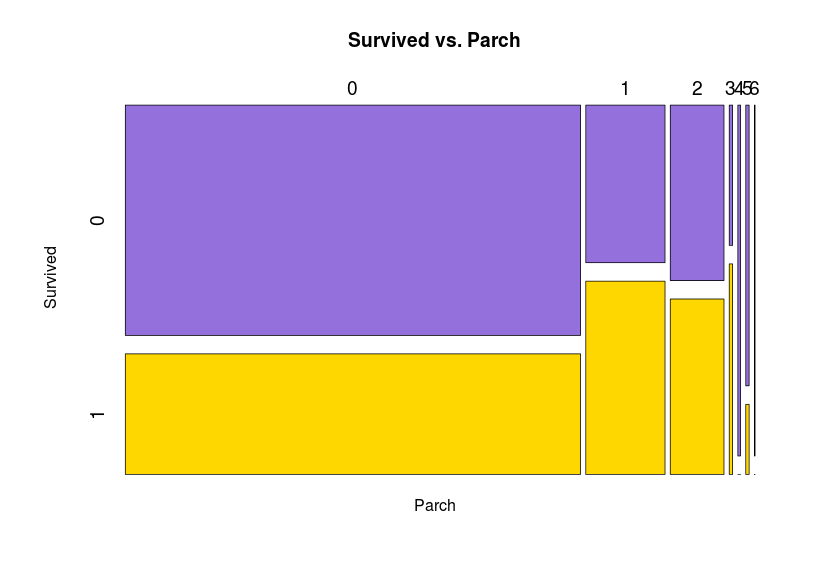
\includegraphics[scale=0.40]{images/survived-vs-parch.png}
\end{center}

\subsection{Opłata}

Na wykresie widać, że wpływ atrybutu nie jest jednoznaczny.
\begin{center}
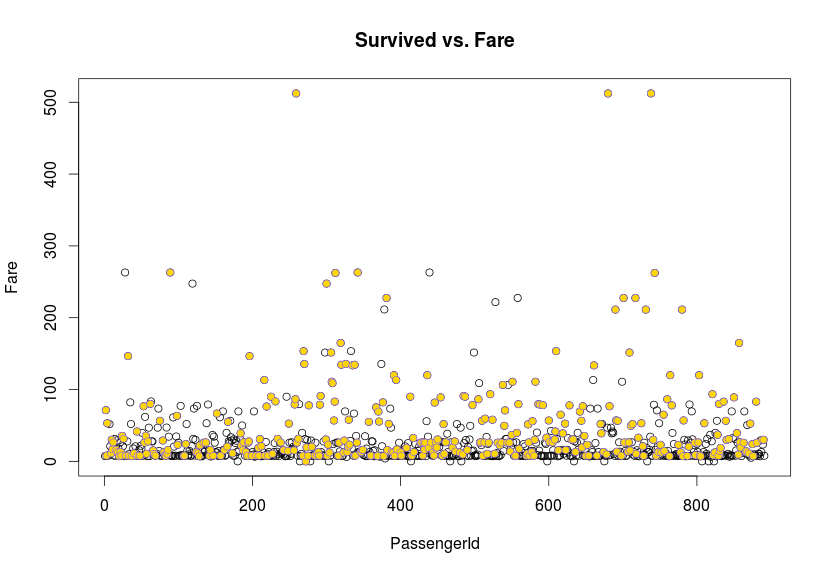
\includegraphics[scale=0.40]{images/survived-vs-fare.png}
\end{center}

TODO Jakimi dwiema zmiennymi?

15 rekordów ma wartość 0, dlatego potraktowaliśmy je jako braki danych, które uzupełniliśmy medianą dla klasy. Poniższy wykres pokazuje zależność między tymi dwiema zmiennymi.
\begin{center}
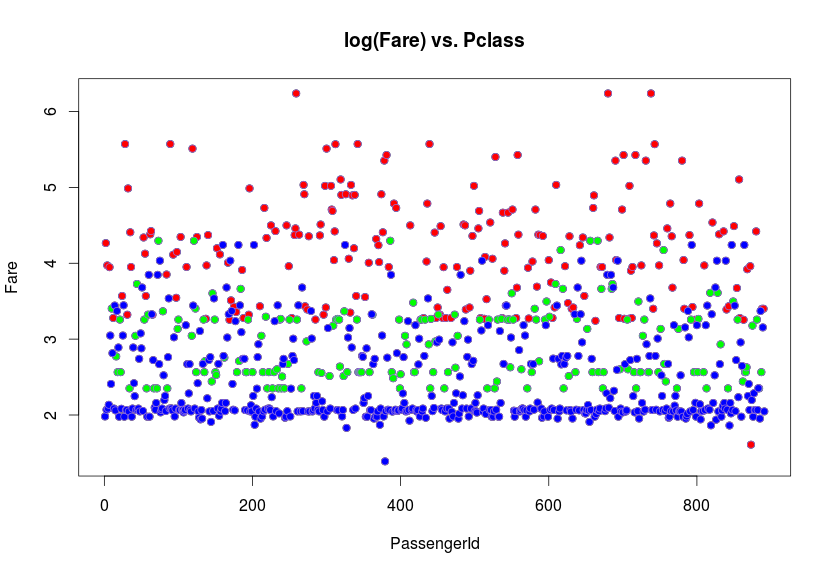
\includegraphics[scale=0.40]{images/logfare-vs-pclass.png}
\end{center}

\subsection{Miejsce wejścia na pokład }

Większość pasażerów okrętowało się w Southampton, dlatego 2 brakujące rekordy zastąpione tym właśnie portem.
\begin{center}
    \begin{tabular}{| l | l | l | l |}
    \hline
        &  C &  Q &  S  \\ \hline
      2 & 168 & 77 & 644  \\
    \hline
    \end{tabular}
\end{center}

Ku naszemu zaskoczeniu, widać, że wartości tego atrybutu posiadają korelację z wpływem na przeżycie osoby podróżującej.

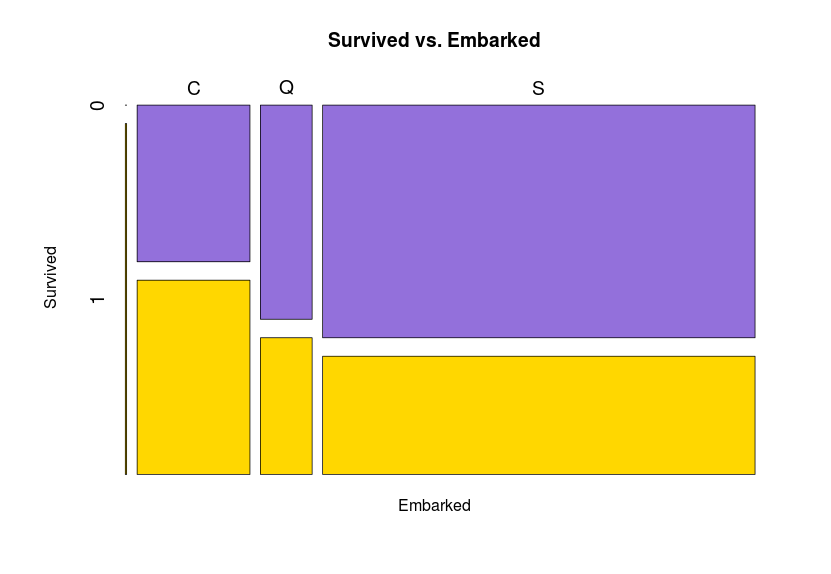
\includegraphics[scale=0.40]{images/survived-vs-embarked.png}

\section{Selekcja atrybutów}
\section{Kalibracja}
\section{Tworzenie modeli}
\section{Ocena jakości modeli}
\section{Podsumowanie}

\end{document}
